%! TeX program = lualatex
\documentclass[12pt,a4paper]{instrukcja}

\begin{document}

\begin{center}
	\vspace*{2cm}

 	\hrulefill
	
	\vspace{0.7cm}
	

		\textbf{\textsc{{\Huge{Obrzędy Wielkiego Tygodnia}}\\\bigskip{\large wg OHS 1955-1962}}}
	
	\vspace{0.5cm}
	
	\hrulefill

	\vspace{\fill}	

	 {\large \textbf{Użyte oznaczenia:}} \\
	
	 \vspace{0.1\textwidth}
	 
	 {\large\centering
	   \begin{itemize}[leftmargin=.43\linewidth,rightmargin=.35\linewidth,label=]
	    \item \ii~ -- celebrans 
	    \item \dd~ -- diakon 
	    \item \ss~ -- subdiakon
 	    \item \cc~ -- ceremoniarze 
	    \item \aa~ -- akolici 
	    \item \tt~ -- turyferarz 
	    \item \ding{63} -- krzyż procesyjny
	    \item \oo -- ombrelino
	  \end{itemize}
	 }
	
	\vspace{5cm}	
	
	\hrulefill
	
	{\footnotesize Pierwsza edycja -- 9 kwietnia 2017\\
	Druga edycja -- 8 kwietnia 2019 \\
	Wszelkie zastrzeżenia proszę kierować do autora na adres: \texttt{michal96.96@gmail.com}}

	\newpage
\end{center}

	

\thispagestyle{empty}

\tableofcontents

% \newpage

\pagestyle{plain}

%! TeX program = lualatex
\documentclass[10pt,a4paper]{instrukcja}

\fancyhead{}
\fancyfoot[C]{Imprimatur 		-- ks. Ireneusz Bakalarczyk}
\fancyfoot[L]{Nihil Obstat		-- Jakub Gajewski}
\fancyfoot[R]{Skład 			-- Michał Siemaszko}

\begin{document}

%%%%%%%%%%%%%%%%%%%%%%%%%%%%%%%%%%

\header{Oczyszczenie NMP}
%%%%%%%%%%%%%%%%%%%%%%%%%%%%%%%%%%
\section{Poświęcenie Gromnic i procesja}

\begin{itemize}
	\item Do prezbiterium wychodzimy normalnie, kapłan ubrany w białą kapę
	\item Po \textit{Dominus vobiscum} następuje 5 oracji po czym zasypanie,
	      pokropienie i okadzenie (potrzebny turyfer i ministrant z kropielnicą)
	      \footnote{\textbf{UWAGA}: może być tak, że celebrans pójdzie pokropić
		      świece wiernych}
	\item Świece rozdawane są ministrantom w sposób podobny do przyjmowania
	      Komunii Św.
	      \footnote{w trakcie rozdawania śpiewa się \textit{Pieśń Symeona}}
	\item Po zakończeniu rozdawania świec następuje ostatnia oracja
	\item Formuje się procesja z krzyżem i akolitami. Idą w niej wszyscy
	      ministranci, celebrans oraz  wierni. Wszyscy mają \underline{zapalone świece}.
	\item Idziemy dookoła kościoła i wracamy do prezbiterium
	\item Po powrocie celebrans zakłada biały ornat i wszyscy gaszą gromnice
\end{itemize}

\section{Zmiany na Mszy Świętej}

\begin{itemize}
	\item Brak modlitw u stopni ołtarza
	\item Msza z dnia bez perturbacji
	\item Zapalamy gromnice na Ewangelię i od \textit{Sanctus} do końca Kanonu.
	\item Zaleca się zrobienie lucenarium
\end{itemize}

\end{document}


\chapter{Pasterka}

\section{Procesja wejścia}

\begin{itemize}
	\item W kościele należy wygasić światła.
	\item Kapłan ubrany w kapę koloru białego bez akompaniamentu organów
	      się do żłóbka ustawionego w prezbiterium. (W tym czasie jeden z
	      usługujących może uderzyć 12 razy w gong)
	\item Po przyjściu kładzie figurkę Dzieciątka i przykrywa ją welonem.
	      Następnie staje przy krześle wraz z asystą.
	\item Kantor staje na ambonie i śpiewa Kalendę: \smallbreak
	      %
	      \inde{Octavo Kalendas Januarii Luna N.\\
		      Innumeris transactis saeculis a creatione mundi, quando in
		      principio Deus creavit caelum et terram et hominem formavit ad
		      imaginem suam;\\
		      permultis etiam saeculis, ex quo post diluvium Altissimus in
		      nubibus arcum posuerat, signum fœderis et pacis;\\
		      a migratione Abrahæ, patris nostri in fide, de Ur Chaldæorum
		      saeculo vigesimo primo;\\
		      ab egressu populi Israël de Ægypto, Moyse duce, saeculo decimo
		      tertio;\\
		      ab unctione David in regem, anno circiter millesimo;\\
		      hebdomada sexagesima quinta, juxta Danielis prophetiam;\\
		      Olympiade centesima nonagesima quarta;\\
		      ab Urbe condita anno septingentesimo quinquagesimo secundo;\\
		      anno imperii Cæsaris Octaviani Augusti quadragesimo secundo;\\
		      toto orbe in pace composito, \textbf{Jesus Christus}, æternus Deus
		      æternique Patris Filius, mundum volens adventu suo piissimo
		      consecrare, de Spiritu Sancto conceptus, novemque post
		      conceptionem decursis mensibus, in Bethlehem Judæ \textbf{nascitur
		      ex Maria Virgine factus homo}:}
	      \smallbreak
	\item[] Tu zapala się światła w kościele.
	      \smallbreak
	      \inde{Nativitas Domini nostri \textbf{Jesu Christi} secundum carnem.}
	      %
	\item Tu bije się we wszystkie dzwonki (podobnie jak w czasie
	      \textit{Gloria} w trakcie Wigilii Paschalnej) i odzywają się organy.
	\item Rozpoczyna się śpiew pieśni Wśród Nocnej Ciszy. Kapłan w tym czasie
	      odkrywa figurkę Dzieciątka, nakłada kadzidło do kadzielnicy i okadza
	      figurkę Dzieciątka. Można też teraz przyozdobić żłóbek kwiatami.
	\item Po zakończeniu śpiewu wszyscy siadają, a kapłan udaje się na ambonę i
	      wygłasza homilię.
	\item Po homilii kapłan ubiera szaty mszalne koloru białego i rozpoczyna
	      Mszę jak zwykle.
\end{itemize}

\section{Zmiany na Mszy Świętej}

\begin{itemize}
	\item Podczas lekcji imię \textbf{Jezus} pada dwa razy -- na oba razy
	      skłaniamy głowę w stronę krzyża
	\item Jeśli wystarczy ministrantów to robimy lucenarium
	\item Jest bożonarodzeniowe \textit{Communicantes}
\end{itemize}


% \footer{
% 	Nihil Obstat	-- Karol Pyziołek 			\hfill 
% 	Imprimatur 		-- ks. Ireneusz Bakalarczyk \hfill 
% 	Skład 			-- Michał Siemaszko}


\chapter{Niedzila Palmowa}

\section{Przygotowanie do obrzędów}
		
		\subsection{W zakrystii}
		
			\begin{itemize}
   				\item dla \ii: humerał, alba z koronką, cingulum białe, stuła i kapa: {\color{red}czerwone},
				\item dla \dd: humerał, alba z koronką, cingulum białe, stuła i dalmatyka: {\color{red}czerwone},
				\item dla \ss: humerał, alba z koronką, cingulum białe, tunicela {\color{red}czerwona},
				\item dla \ding{63}: tunicela {\color{red}czerwona},
				\item akolitki,
				\item kadzielnica z łódką, 
			\end{itemize}
		
		\subsection{Na kredensji w kościele}
		
			\begin{itemize}
				\item kielich do Mszy św. z wszystkimi paramentami barwy  {\color{violet}fioletowej} (w tym welon naramienny dla \ss),
				\item tacka z ampułkami i ręcznikiem do Mszy św.,
				\item dzwonek,
				\item 2 pateny,
				\item 2 świeczki \textit{Sanctusowe},
%				\item księga OHS, 
				\item lekcjonarz,
				\item teksty pasji z nutami (po polsku),
			\end{itemize}
		
%			W miarę możliwości kielich i paramenta {\color{violet}fioletowe} do chwili zakończenia procesji powinny być zakryte {\color{red}czerwoną} zasłoną.
			
		\subsection{Na ołtarzu polowym}
			
			\begin{itemize}
				\item krzyż,
				\item 6 świec z osłonkami,
				\item księga OHS ubrana we {\color{violet}fioletową} okładkę,
				\item pulpit albo poduszka na OHS,
			\end{itemize}
		
		\subsection{Na kredensji na dworze}
			
			\begin{itemize}
				\item naczynie z wodą święconą i kropidło,
				\item ewangeliarz ubrany w {\color{red}czerwoną} okładkę,
%				\item lekcjonarz dla diakona do śpiewania,
				\item mydło, miska i dzbanek z wodą do umycia rąk celebransa po rozdaniu palm,
				\item ręcznik,
%				\item teksty do recytowania podczas procesji,
				\item miejsce na akolitki,
				\item miejsce na birety,
			\end{itemize}
		
		\subsection{Na Sedilli w kościele}
		
			\begin{itemize}
				\item dla \ii~ manipularz, stuła i ornat – {\color{violet}fioletowe},
				\item dla \dd~ manipularz, stuła i dalmatyka – {\color{violet}fioletowe},
				\item dla \ss~ manipularz i tunicela – {\color{violet}fioletowe},
			\end{itemize}
	
		\subsection{Po stronie ewangelii}
			
			\begin{itemize}
				\item trzy wysokie pulpity bez nakrycia do śpiewania pasji \footnote{ustawione na północ chyba że nie uda się zorganizować mikrofonów},
				\item przynajmniej jeden mikrofon.
			\end{itemize}

\section{Procesja wejścia}

\begin{itemize*}
	\item Standardowa procesja wejścia. Jeśli jest \ding{63}, idzie on między
	      \aa~. \tt~ niesie trybularz i łódkę. \cc2 idzie w parze z \tt. \ii~ ubrany
	      jest w fioletową kapę.
	\item Liturgia może rozpocząć się od kazania (jak w 2019 roku).
\end{itemize*}

\section{Uroczyste modły}

\begin{itemize}
      \item \zz~ przynosi z zakrystii czarną kapę
      \item \ii~ zakłada czarną kapę przy pomocy \cc1 i \cc2
      \item  w tym czasie \aa1 oraz \aa2 rozkładają na ołtarzu jeden obrus oraz
            ustawiają na środku pulpit z mszałem oraz kartką z wezwaniem
            modlitwy powszechnej za żydów, potem wracają na swoje miejsca przy
            kredencji
      \item  \ii~ wraz z \cc1 i \cc2 przytrzymującymi brzegi kapy podchodzi
            przed ołtarz, wykonują ukłon i wchodzą na stopnie
      \item  \ii~ całuje mensę ołtarzową i rozpoczyna śpiew modlitw
      \item  na wezwanie \textit{Flectamus genua} wszyscy klękają, na
            \textit{Levate} – wstają
      \item  po zakończeniu modlitw \ii~, \cc1 i \cc2 skłaniają głowy i wracają
            do sedilli krótką drogą, \cc1 i \cc2 trzymają kapę
      \item \tt1 zabiera mszał wraz ze stojakiem z ołtarza
      \item  \ii~ zdejmuje kapę, którą Z odnosi do zakrystii
\end{itemize}

\section{Dodatek}
\label{sec:dodatek_palm}

\subsection[Losy subdiakona krucyfera]{Losy subdiakona krucyfera \protect \footnote{Wymagany level -- obłuczony kleryk}}
\begin{itemize}
      \item subdiakon krucyfer ( \ding{63} ), ubrany w albę, cingulum i czerwoną
            tunicellę
      \item nie odbiera palmy od \ii
      \item po skończonej procesji idzie do kaplicy zimowej, gdzie ściąga westymenta
            subdiakona, zakłada komżę, bierze biret i przechodzi do chóru
\end{itemize}

\subsection{Procesja do Ewangelii - dla zaawansowanych}

\subsubsection*{\textbf{Celebrans z subdiakonem i ceremoniarzem }}
\begin{itemize}
      \item kiedy skończy się śpiew \textit{Graduału} i \textit{Traktusa}, \ii~ wraz
            z \ss~ i \cc1 podchodzą do ołtarza - przyklękają
      \item \ii~ wchodzi na najwyższy stopień i odmawia modlitwę \textit{Munda cor}
      \item \ss~ w tym czasie przenosi mszał
      \item \ss~ przechodzi ze Mszałem na stronę Ewangelii i pozostaje przy nim
            asystując \ii~ przy kartkach
      \item \cc1, \tt, \aa1, \aa2 \textbf{nie} ustawiają się jak na Mszy
            śpiewanej (zostają na swoich bazach) \footnote{Ceremoniał o.
                  Małaczyńskiego, str. 65, pkt. 47(dla rytu uroczystego): „Jeżeli Męka
                  Pańska nie jest śpiewana celebrans pod koniec traktusa odmawia
                  \textit{Munda cor} i czyta Mękę Pańską po stronie Ewangelii.
                  Równocześnie należy ją odczytać wiernym  po polsku."}
      \item \ii~ po przeczytaniu Pasji nie schodzi do sedilli tylko idzie na
            stronę lekcji i obraca się w kierunku śpiewanej pasji; \ss~ stoi na
            swoim stopniu (\textit{in plano}) po stronie lekcji odwrócony w
            stronę pasji, mogą wziąć palmy
\end{itemize}

\subsubsection*{\textbf{Diakon i śpiewacy}}
\begin{itemize}
      \item \dd, przy pomocy \cc2, zdejmuje dalmatykę i manipularz
      \item \dd, od \cc2, otrzymuje księgę z tekstem Pasji
      \item \cc2 prowadzi \dd~ do ambony, \eighthnote1 i \eighthnote2 czekają na
            miejscu; śpiew pasji wykonywany jest po stronie ewangelii przed
            balaskami
      \item wszystkie skłony podczas Pasji wykonujemy w stronę
            ewangeliarza/lekcjonarza (nie w stronę Mszału),
      \item po skończonej Pasji \dd~ i \cc2 przyklękają na środku, po czym \cc2
            prowadzi \dd~ do sedilli i pomaga mu założyć dalmatykę i manipularz
      \item \dd~ zajmuje swoje miejsce za \ii~ i przyklęka --
            \ii~ rozpoczyna \textit{Credo}
\end{itemize}

\section{Dodatek}

\subsection{Przebieg poświęcenia wody}
\label{sec:woda}
\begin{enumerate}
      \item \textit{Dominus Vobiscum} i Oracja 0. (przed wejściem)
            \smallfont{(złożone ręce)}
      \item \textit{Dominus Vobiscum} i Oracja 1. \smallfont{(złożone ręce)}
      \item Prefacja do słów \textit{Sumat unigeniti tui gratiam de Spiritu
                  Sancto}
      \item Celebrans kreśli znak krzyża
            \textcolor{red}{\raisebox{-1mm}{\scalebox{1.5}{\ding{64}}}} na
            wodzie
      \item Wyciera ręce
      \item Kontynuuje modlitwę
      \item Na \textit{Sit haec} kładzie rękę na powierzchni wody
      \item Wyciera rękę
      \item Kreśli znaki krzyża
            \textcolor{red}{\raisebox{-1mm}{\scalebox{1.5}{\ding{64}}}}
            nad wodą na słowa \textit{Per Deum vivum \dots}
            \vspace*{-11pt}
      \item Wylewa wodę na cztery strony świata po słowach \textit{... super te
                  ferebatur} ~~~
            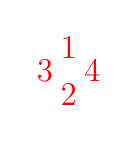
\begin{tikzpicture}[scale=0.3, baseline=-1mm, thick]
                  \draw[color=red] (10mm,0) node {\large 4};
                  \draw[color=red] (-10mm,0) node {\large 3};
                  \draw[color=red] (0,10mm) node {\large 1};
                  \draw[color=red] (0,-10mm) node {\large 2};
            \end{tikzpicture}
            \vspace*{-7pt}
      \item Kreśli znak krzyża nad wodą na \textit{Benedico te}
      \item Po zmianie głosu na \textit{recto tono} na słowa \textit{tu benignus
                  aspira} trzy razy dmucha do wody na kształt krzyża
      \item W tym czasie ceremoniarz podaje Paschał
      \item Na słowa \textit{Descendad in hanc} trzy razy wkłada Paschał do wody
            i śpiewa \footnote{Wkłada Paschał coraz głębiej}
      \item \ii~ trzy razy dmucha do wody w kształcie litery
            \textcolor{red}{\raisebox{-1mm}{\Large ${\Psi}$}} i kontynuuje
            \textit{Totamque ... effectu}
      \item Wyciągamy Paschał z wody i kończymy święcenie wody (\textit{... per
                  ignem.})
      \item Po wyjęciu paschału nabiera się wody do pokropienia
      \item Następnie \cc1 przynosi do chrzcielnicy tackę z olejami świętymi i
            wręcza \ii~ (z pocałunkiem) odpowiednie ampułki. \ii, wypowiadając
            słowa przepisane w księdze po kolei:
            \begin{itemize}
                  \item wlewa olej katechumenów
                  \item wlewa krzyżmo
                  \item wlewa oba
            \end{itemize}
      \item Następnie miesza wodę ręką lub przy pomocy łyżeczki
      \item Później myje i wyciera ręce \footnote{W razie potrzeby wykorzystuje
                  sól, watę i miękisz chleba, które później należy spalić. Wodę
                  z tej ablucji wlewa
                  się do sacrarium.}
\end{enumerate}

\subsection{Bierzmowanie}
\label{sec:bierz}
\begin{itemize}
      \item księgę z modlitwami trzyma \cc1, a \cc2 podtrzymuje kapę jeśli
            trzeba; \aa1 i \aa2 stoją z boku przy kredencji
      \item \ii~ odmawia modlitwę zwracając się do kandydatów \textit{Spiritus
                  Sanctus superveniat\dots}
      \item \ii~ czyni znak Krzyża Świetego mówiąc \textit{Adjutorium
                  nostrum...} a następnie kontynuowany jest krótki dialog
      \item \ii~ wyciąga ręce nad przystępującymi do bierzmowania i mówi
            \textit{Oremus. Omnipotens sempiterne Deus,...}
      \item przystępujący do sakramentu klęka przed \ii. Świadek kładzie rękę na
            prawym ramieniu bierzmowanego.
      \item \aa1 podchodzi do \ii~ z Krzyżmem Świętem
      \item \ii~ kładzie prawą rękę na głowie bierzmowanego i palcem umoczonym w
            Krzyżmie Świętym robi znak krzyż a na czole, mówiąc \textit{Signo te
                  signo...}
      \item \ii~ uderza lekko w policzek bierzmowanego, mówiąc \textit{Pax tecum}
      \item kandydat wraca na swoje wcześniejsze miejsce i stoi
      \item \aa1 odbiera Krzyżmo, a \aa2 podchodzi z czymś do wytarcia palców
            \footnote{najpewniej wata}; później wracają do kredencji
      \item gdy \ii~ namaści wszystkich kandydatów, śpiewa się antyfonę
            \textit{Confirma hoc, Deus\dots}
      \item powtarza się antyfonę, a następnie \ii~ zwrócony do ołtarza śpiewa
            \textit{Ostende nobis, Domine,...}, a następnie \textit{Oremus.
                  Deus, qui Apostolis tuis\dots}
      \item \ii~ mówi \textit{Ecce sic benedicetur omnis homo, qui timet Dominum}
      \item na końcu \ii~ błogosławi bierzmowanych
            \textit{Bene} + \textit{dicat vos Dominus ex Sion...}
\end{itemize}

\color{red}

\section{Uwagi}
\begin{itemize}
      \item można zrobić jakieś święcenie ognia przed proroctwami tak aby ludzie
            oświetlali kościół i mieć jakąś namiastkę Wigilii Paschalnej
      \item na poświęcenie wody ludzie \textbf{muszą mieć zapalne świece}
      \item zapytać księdza czy będzie aspersja (czy to humanitarne?)
      \item ziomek do chrztu musi siedzieć za kratą aż do ochrzczenia -- trzeba
            mu przygotować jakieś krzesło i klęcznik
      \item na chrzest dorosłego ksiądz ubiera kapę (patrz Nowowiejski)
\end{itemize}

\chapter{Uroczyste Requiem}

\section{Przygotowanie}%

\begin{itemize}
	\item Ołtarz główny:
		\begin{itemize}
			\item bez kwiatów
			\item mszał otwarty
			\item katafalk
			\item 4 świeczniki z \textcolor{orange}{żółtymi} świecami
			\item przy sedilli dodatkowe dwa miejsca dla akolitów
			\item \textbf{czarne} antepedium
		\end{itemize}
	\item Kredencja:
		\begin{itemize}
			\item kielich nakryty \textbf{czarnym} welonem
			\item brak welonu naramiennego dla \ss
			\item ampułki
			\item lawaterz, ręczniczek
			\item dzwonki
			\item lekcjonarz/ewangeliarz
			\item dwie pateny komunijne
			\item dwie świece sanctusowe
			\item kociołek, aspergil
			\item rytuał
		\end{itemize}
	\item Zakrystia/kaplica:
		\begin{itemize}
			\item dla \ii: humerał, alba simplex, \textbf{czarne
				cingulum, czarny ornat, stuła, manipularz},
				biret
			\item dla \dd: humerał, alba simplex, \textbf{czarne cingulum,
				czarna dalmatyka, stuła, manipularz}, biret
			\item dla \ss: humerał, alba simplex, \textbf{czarne cingulum,
				czarna tunicella, (manipularz)}, biret
			\item \textbf{czarna kapa}
			\item krzyż procesyjny
			\item trybularz, łódka
			\item akolitki (z \textcolor{orange}{żółtymi} świecami)
		\end{itemize}
\end{itemize}

\section{Pochód do ołtarza}

\begin{itemize}
	\item procesja wejścia przebiega w następującym porządku:
		\begin{center}
			\tt~~~\cc2 \\
			\aa2 ~~ \ding{63} ~~ \aa1\\
			ministranci\\
			\cc1 \\
			\ss \\
			\dd \\
			\ii 
		\end{center}
    \item \aa\aa~ wnoszą zapalone akolitki w procesji wejścia oraz wynoszą po
	    zakończeniu mszy; w czasie mszy akolitki stoją zapalone na
	    kredencji i nie są używane na Ewangelię
    \item \tt~ nie wnosi kadzielnicy w procesji wejścia
    \item \ii, \dd~ i \ss~ oddają birety \cc1, a następnie przyklękają na jego znak
    \item podczas mszy opuszcza się wszystkie pocałunki
\end{itemize}

\section{Od modlitwy u stopni do sekwencji}

\begin{itemize}
	\item  \cc1 daje znak dla asysty do klęknięcia
	\item następują modlitwy u stopni z pominięciem psalmu 42 \textit{Iudica me}
	\item \ii~wstępuje po stopniach ołtarza i go całuje
	\item pomija się okadzenie, przejście od razu na \textit{Introit}
	\item \ii~kładzie lewą rękę na ołtarzu, a prawą czyni znak krzyża nad
		otwartym mszałem; czyta \textit{Introit}
	\item cała asysta opuszcza znak krzyża
	\item \ii, \dd, \ss~i \cc1 recytują \textit{Kyrie}	
	\item po zakończeniu recytacji \dd~i \ss~stają za \ii, a jeśli śpiew się
		przedłuża schodzą krótką drogą do sedilli
	\item pod koniec Kyrie \ii, \dd~i \ss~przechodzą na środek
	\item \ii~całuje ołtarz, śpiewa pozdrowienie i razem z \dd~i \ss~przechodzą
		na stronę lekcji
	\item podczas kolekty, od \textit{Dominus Vobiscum} aż do
		\textit{Amen}, cała asysta niższa klęczy
	\item pod koniec oracji \cc1 zabiera z kredencji lekcjonarz i przekazuje
		go \ss
	\item \cc1 i \ss~przyklękają na osi ołtarza i odchodzą na miejsce śpiewania
		lekcji, gdzie \cc1 staje po lewej stronie \ss~(bliżej osi ołtarza)
	\item \dd~zajmuje miejsce przy mszale
	\item \ss~śpiewa lekcję, którą \ii~czyta cicho w mszale
	\item \ss~wraca z \cc1, przyklękają na osi ołtarza
	\item \cc1 odbiera lekcjonarz, \ss~nie podchodzi po błogosławieństwo, tylko
		razem z \dd~stają jak na \textit{Introit}
	\item \ii~recytuje sekwencję, \cc1 asystuje przy mszale
	\item po zakończeniu recytacji asysta wyższa schodzi krótką drogą do
		sedilli
	\item około słów \textit{Qui Mariam absolvisti}, na znak \cc1 wracają do ołtarza
		przyklękając na środkui
	\item \ii~wchodzi po stopniach i staje pośrodku ołtarza
\end{itemize}

\section{Ewangelia}

\begin{itemize}
	\item \cc1 podaje \dd~ewangeliarz
	\item w tym czasie \ss~wchodzi na suppedaneum po stronie lekcji, skąd
		zabiera mszał i wraca z nim przed stopnie, po lewej stronie \dd
	\item \dd~i \ss~przyklękają i wchodzą po stopniach, każdy na swoją stronę
	\item \ss~stawia mszał po stronie ewangelii, a \dd~kładzie ewangeliarz na
		środku ołtarza
	\item w tym czasie przed ołtarzem ustawiają się \aa1, \aa2 (bez akolitek),
		\tt~(bez kadzielnicy) oraz \cc1
	\item \ss~schodzi przed stopnie i zajmuje miejsce w pierwszym rzędzie po
		stronie ewangelii
	\item \dd~klęka na skraju suppedaneum, na prawo od \ii~i odmawia
		\textit{Munda cor meum}, następnie wstaje, zabiera ewangeliarz,
		skłania się i nie prosząc o błogosławieństwo schodzi przed
		stopnie po stronie lekcji; porządek wygląda następująco:
		\begin{center}
			|\_\_\_\_\_\_\_\_\_\_\_\_\_\_\_\_\_\_\_\_\_\_\_\_\_\_|\\
			\ss~~~~\dd\\
			\cc1~~~~\tt\\
			\aa2~~~~\aa1
		\end{center}
	\item wszyscy przed stopniami przyklękają i odchodzą na miejsce proklamacji
		ewangelii, gdzie ustawiają się jak zwykle
	\item pomija się okadzenie, \dd~rozpoczyna śpiew Ewangelii
	\item po zakończeniu proklamacji nie okadza się celebransa
	\item \ss~oddaje ewangeliarz \cc1 
	\item wszyscy wracają przed ołtarz w tym samym porządku
	\item na znak \cc1 przyklękają i wracają na swoje miejsca: \dd~i \ss~na stopniach
		za \ii, \aa\aa~ do kredencji, \tt~idzie przygotować kadzielnicę (która
		powinna być rozpalona już wcześniej), a \cc1 odnosi ewangeliarz na
		kredencję i staje na swoim miejscu
	\item w tym miejscu liturgii nie przewiduje się kazania
\end{itemize}

\section{Ofiarowanie}

\begin{itemize}
	\item \ii~całuje ołtarz i śpiewa \textit{Dominus vobiscum} oraz
		\textit{Oremus}
	\item \dd~wchodzi na suppedaneum i staje po prawej stronie \ii~(bez
		przyklęknięcia)
	\item \ss~i \cc1 przyklękają na środku i odchodzą do kredencji
	\item \ss~bierze kielich przykryty welonem i bursą, i zanosi go na
		ołtarz, sam jednak nie zakłada welonu naramiennego, gdyż nie
		trzyma pateny
	\item \dd~rozkłada korporał na ołtarzu, \ss~rozbiera kielich
	\item \aa1 przynosi na ołtarz ampułki, odbiera od \ss~welon kielichowy i
		odnosi go na kredencję
	\item jeśli może, \ss~nalewa wody do kielicha, jeśli nie, robi to \dd, w
		obu przypadkach jednak nie prosząc \ii~o błogosławieństwo
	\item \aa1 zabiera ampułki z ołtarza na kredencję
	\item \tt~przychodzi z rozpaloną kadzielnicą i łódką
	\item \ss~nie trzyma pateny, więc przechodzi na lewą stronę \ii,
		przyklękając na środku na najniższym stopniu
	\item \dd~chowa patenę pod korporałem, jak na mszy śpiewanej
	\item następuje okadzenie; \cc1 odbiera łódkę od \tt~i razem wchodzą po
		stopniach
	\item \cc1 podaje łódkę \dd, następuje zasypanie
	\item \dd~oddaje łódkę \cc1, a odbiera kadzielnicę od \tt
	\item \cc1 i \tt~schodzą ze stopni
	\item okadzenie ołtarza przebiega jak zwykle
	\item \cc1 przechodzi na stronę ewangelii i w odpowiedniej chwili ściąga
		z ołtarza mszał, po okadzeniu odnosi go i zostaje przy mszale
	\item po okadzeniu ołtarza okadzony zostaje jedynie \ii~(przez \dd~i \ss)
	\item \tt~wynosi kadzielnicę bez dalszych okadzeń, idzie na środek
		i czeka aż dołączą do niego ceroferariusze wraz z \cc2
	\item \cc2 wyprowadza ceroferariuszy (dwóch lub czterech), którzy idą
		przygotować pochodnie – przyklękają parami na środku i odchodzą
	\item \dd~i \ss~stają w linii za \ii~(jak na oracje)
	\item \aa\aa~ dokonują obmycia rąk \ii~(lavabo)
	\item \ii, \dd~i \ss~przechodzą na środek, wciąż stojąc w linii
	\item \dd~odpowiada na \textit{Orate, fratres}
\end{itemize}

\section{Prefacja i Kanon Rzymski}

\begin{itemize}
	\item następuje prefacja
	\item pod koniec prefacji \cc1 skłania się do \dd~i \ss, po czym odchodzi od
		mszału i idzie na swoje miejsce
	\item \dd~i \ss~wchodzą na suppedaneum i pochyleni recytują \textit{Sanctus}
		razem z \ii~(\dd~po prawej, \ss~po lewej przy mszale)
	\item po zakończeniu recytacji \dd~i \ss~stają na stopniach za \ii~i
		przyklękają
	\item \dd~przechodzi na stronę ewangelii i asystuje przy mszale
	\item \ss~zostaje przed najniższym stopniem i stoi tam ze złożonymi rękami
	\item do ołtarza przychodzą \cc2, \tt~oraz ceroferariusze
	\item przyklękają na środku, \tt~odchodzi do kredencji, a \cc2 na swoje
		miejsce
	\item w czasie Kanonu Rzymskiego cała asysta niższa klęczy – od
		zakończenia recytacji \textit{Sanctus} aż do końcowego
		\textit{Amen}, dlatego na znak \cc2 wszyscy klękają na oba
		kolana, w tym ceroferariusze na środku \item na słowa \textit{Quam
		oblationem} \dd~schodzi na środek, przyklęka i przechodzi na
		prawą stronę \ii
	\item w tym czasie \ss, nie przyklękając, przechodzi wzdłuż stopni na
		stronę lekcji, gdzie odbiera przy kredencji zasypaną
		kadzielnicę od \tt, a następnie klęka na najniższym stopniu; \cc1
		klęka w tym samym momencie
	\item podczas podniesienia \ss~okadza Najświętszy Sakrament
	\item po konsekracji \dd~wraca do mszału na lewą stronę \ii, z
		przyklęknięciami po obu stronach, natomiast \ss~oddaje
		kadzielnicę \tt~i wraca na środek, gdzie przyklęka i stoi aż do
		\textit{Pax Domini sit semper vobiscum}
	\item jak zwykle po słowach \textit{Nobis quoque peccatoribus} \dd~przyklęka przy
		mszale, przechodzi na prawą stronę \ii~i znów przyklęka
	\item \cc1 przechodzi na środek, przyklęka (za plecami \ss) i zajmuje
		miejsce przy mszale, gdzie znów przyklęka (równocześnie z \dd)
	\item po zakończeniu Kanonu wszyscy wstają na znak \cc2
	\item ceroferariusze przyklękają na środku razem z \cc2 i \tt, a następnie
		razem z nimi wychodzą
\end{itemize}

\section{Od \textit{Pater Noster} do końca Mszy}

\begin{itemize}
	\item \ii~rozpoczyna śpiew \textit{Pater noster}, \dd~przyklęka,
		schodzi na stopień za \ii~i tam znów przyklęka
	\item na słowa \textit{Et dimitte nobis} \dd~przyklęka, wraca na prawą
		stronę \ii~i bez pocałunku podaje mu patenę; w tym czasie
		\ss~pozostaje na swoim miejscu
	\item na słowa \textit{Pax Domini sit semper vobiscum} \ss~i \cc1 przyklękają, a
		następnie \ss~zajmuje miejsce przy mszale, \cc1 zaś odchodzi na
		swoje miejsce
	\item \ii, \dd~i \ss~recytują \textit{Agnus Dei} w zmienionej formie,
		stąd nie biją się w pierś
	\item opuszcza się przekazanie pocałunku pokoju, więc po zakończeniu
		recytacji \dd~i \ss~zamieniają się miejscami przyklękając przed i
		po
	\item \cc2, \tt~i ceroferariusze wracają do ołtarza i razem z pozostałymi
		ministrantami formują procesję komunijną
	\item \cc1 daje znak do przyklęknięcia, a następnie do klęknięcia
	\item następuje komunia wiernych
	\item po komunii \aa1 zanosi na ołtarz ampułki, a po ablucjach je zabiera
	\item \dd~bierze mszał, który przenosi na stronę lekcji, \ss~bierze palkę,
		którą przenosi na stronę ewangelii, przyklękają na środku na
		swoich stopniach
	\item \aa2 zanosi welon kielichowy na stronę ewangelii i podaje go \ss
	\item \cc1 przechodzi do mszału
	\item \ss~odnosi kielich na kredencję
	\item \ii, \dd~i \ss~stają w jednej linii, następuje \textit{Communio},
		wezwanie (na środku) i pokomunia (znów po stronie lekcji)
	\item \cc1 zamyka mszał
	\item \ii, \dd~i \ss~wracają na środek, \ii~całuje ołtarz i śpiewa
		\textit{Dominus vobiscum}
	\item \dd~wciąż zwrócony w stronę ołtarza śpiewa \textit{Requiescant in
		pace}, na co odpowiada się \textit{Amen}
	\item \ii~odmawia \textit{Placeat}, pomija się błogosławieństwo i Ostatnią
		Ewangelię, ponieważ następują absolucje
\end{itemize}

\section{Absolucje}

\begin{itemize}
	\item \ii, \dd~i \ss~odchodzą do sedilli
	\item \zz~ przynosi z zakrystii \textbf{czarną kapę}
	\item \dd~i \ss~z pomocą \zz~ asystują \ii~przy zdejmowaniu ornatu i manipularza
		oraz zakładaniu kapy
	\item \dd~i \ss~zdejmują manipularze z pomocą \aa\aa~
	\item \aa\aa~ biorą akolitki, krucyferariusz podaje krzyż procesyjny \ss
	\item M1 bierze rytuał, M2 bierze kropidło
	\item \tt~przychodzi z kadzielnicą
	\item \ss~trzymając krzyż staje z \aa\aa~ u wezgłowia katafalku, pozostawiając
		odstęp
	\item M1, M2 oraz \tt~stają przy stopniach ołtarzowych po stronie lekcji,
		zwróceni w stronę nawy
	\item \ii~staje w nogach katafalku, mając \dd~po swojej prawej, a \cc1 po
		lewej stronie, zwróceni w stronę nawy (patrz Rys.
		\ref{fig:requiem})
		\begin{figure}[h]
			\centering
			\includegraphics[width=0.8\textwidth]{Figures/requiem.jpg}
			\caption{Ustawienie przy katafalku}
			\label{fig:requiem}
		\end{figure}
	\item ponieważ nie ma ciała, opuszcza się modlitwę \textit{Non intres}
	\item schola rozpoczyna śpiew responsorium \textit{Libera me}
	\item podczas powtórzenia pierwszego wersetu następuje zasypanie
		kadzidła
	\item \tt~oraz \cc1 przechodzą razem na stronę ewangelii
	\item \tt~podaje łódkę \dd~i podnosi kadzielnicę do zasypania
	\item \dd~prosi \textit{Benedicite, Pater reverende}
	\item \ii~zasypuje 3 razy, błogosławiąc w zwykły sposób (bez pocałunków)
	\item \tt~odbiera łódkę i wraca z kadzielnicą na swoje miejsce
	\item \cc1 wraca na lewą stronę \ii
	\item po responsorium śpiewa się dialog \textit{Kyrie, eleison}
	\item M1 podchodzi z rytuałem, staje na prawo od \ii, przed \dd
	\item \ii~zwraca się do zgromadzonych i wspólnie recytują \textit{Ojcze
		nasz}
	\item M1 odchodzi, podchodzi M2 z kropidłem, które podaje \dd
	\item \dd~bez pocałunków podaje kropidło \ii
	\item \dd~trzyma prawą połę kapy, \ii~zaś kropi katafalk najpierw
		trzykrotnie z prawej strony (od strony ewangelii), nie
		zatrzymując się
	\item przechodząc przed krzyżem \ii~ lekko się skłania, a \dd~przyklęka
	\item \ii~kropi katafalk trzykrotnie z lewej strony, również się nie
		zatrzymując
	\item po powrocie przed ołtarz obaj przyklękają przed Najświętszym
		Sakramentem
	\item ustawiają się na powrót przed katafalkiem, \ii~oddaje kropidło \dd, a
		ten M1
	\item M1 odchodzi z kropidłem, podchodzi \tt~z kadzielnicą
	\item \tt~podaje kadzielnicę \dd, a ten \ii
	\item okadzenie następuje analogicznie do pokropienia
	\item podchodzi M1 z rytuałem, \ii~śpiewa wezwania oraz modlitwę
		\textit{Absolve}
	\item \ii~prawą ręką czyni znak krzyża nad katafalkiem i śpiewa wezwania
	\item na zakończenie śpiewa się antyfonę \textit{Salve, Regina}
	\item \ss~oddaje krzyż krucyferariuszowi
	\item ustawia się procesja do wyjścia, w porządku analogicznym jak na
		wejście
\end{itemize}


\end{document}
